\documentclass[../../../include/open-logic-section]{subfiles}

\begin{document}

\olfileid{sth}{ordinals}{idea}	
\olsection{في المعنى العام للعدد الترتيبي}

تأمل الأعداد الطبيعية على ترتيبها المألوف:
\begin{center}
	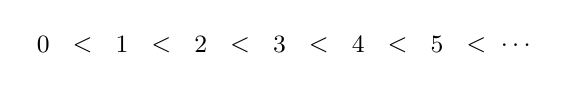
\begin{tikzpicture}
	\foreach \x/\xtext in {0, 1, 2, 3, 4, 5}
	{
		\node (\x a) at (\x, 1) {\small{$\x$}};
		\node (\x a) at (\x.5, 1) {\small{$<$}};
	}
	\node (ldots) at (6, 1) {\small{$\ldots$}};
	\end{tikzpicture}
\end{center}
وهذه، في الاصطلاح، متتالية من النمط~$\omega$؛ وقد ظهر ترتيبها نفسه في
بنائنا الأول لمراحل هرم المجموعات. ولننقل الآن~${\OLMathNumeral{0}}$ إلى آخر المتتالية
بعد سائر الأعداد:
\begin{center}
	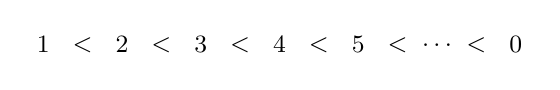
\begin{tikzpicture}
	\foreach \x/\xtext in {1, 2, 3, 4, 5}
	{
		\node (\x a) at (\x, 1) {\small{$\x$}};
		\node (\x a) at (\x.5, 1) {\small{$<$}};
	}
	\node (ldots) at (6, 1) {\small{$\ldots$}};
	\node (bea) at (6.5, 1) {\small{$<$}};
	\node (noa) at (7, 1) {\small{${\OLMathNumeral{0}}$}};
	\end{tikzpicture}
\end{center}
فالكيانات باقية بأعيانها، وإنما تبدل ترتيبها تبدلًا جوهريًا: لم يكن
للترتيب الأول آخر، ولهذا الترتيب آخر. فهو متتالية من النمط~$\omega$
تتألف من (${\OLMathNumeral{1}}, {\OLMathNumeral{2}}, {\OLMathNumeral{3}}, {\OLMathNumeral{4}}, {\OLMathNumeral{5}}, \ldots$)، ثم يتلوها كيان زائد؛ ولذلك هو
متتالية من النمط~$\omega+{\OLMathNumeral{1}}$.

ومن هذه الكيانات نفسها نصنع أنماطًا أخرى. فرتب الأعداد الزوجية كلها
ترتيبها الطبيعي، ثم ألحق بها الأعداد الفردية كلها بترتيبها الطبيعي:
\begin{center}
	\begin{tikzpicture}
	\node(a1) at (1,1) {\small{${\OLMathNumeral{0}}$}};
	\node(a2) at (1.5,1) {\small{$<$}};
	\node(a3) at (2,1) {\small{${\OLMathNumeral{2}}$}};
	\node(a4) at (2.5,1) {\small{$<$}};
	\node(a5) at (3,1) {\small{${\OLMathNumeral{4}}$}};
	\node(a6) at (3.5,1) {\small{$<$}};
	\node(dots) at (4,1) {\small{$\ldots$}};
	\node(aaoe) at (4.5,1) {\small{$<$}};
	\node(b1) at (5,1) {\small{${\OLMathNumeral{1}}$}};
	\node(b2) at (5.5,1) {\small{$<$}};
	\node(b3) at (6,1) {\small{${\OLMathNumeral{3}}$}};
	\node(b4) at (6.5,1) {\small{$<$}};
	\node(b5) at (7,1) {\small{$\ldots$}};
	\end{tikzpicture}
\end{center}
فهذه متتالية نمطها~$\omega$ تليها أخرى نمطها~$\omega$؛ أي إن نمط
المجموع~$\omega+\omega$.

ويمكن متابعة الإنشاء، غير أن غرضنا قاعدة عامة نفهم بها هذا القول في
\emph{الترتيبات}.

\end{document}



